
\begin{problem}
Construct a geometric example showing a compact set $\mathcal{A}$
that does not have a uniqe best approximation to a point in $\mathds{R}^n$.
\end{problem}

\begin{solution}
  The property we need from
  
%% \begin{figure}
%% \includegraphics[scale=2]{drawing_task_1}
%% \end{figure}

\end{solution}

 	

%%% Local Variables:
%%% TeX-master: "report.tex"
%%% End:
